%!TEX root = main.tex

\chapter{FUNDAMENTOS DA TEORIA DOS CONJUNTOS}
\label{chap:fundamentos_teoria_conjuntos}

Neste capítulo, estabelecem-se as bases formais sobre as quais todo o trabalho se sustenta. A Teoria dos Conjuntos fornece a linguagem universal da matemática moderna, mas sua construção requer rigor para evitar contradições. Serão apresentados os axiomas essenciais que definem o comportamento dos conjuntos e suas operações elementares, além da construção axiomática dos números naturais via Axiomas de Peano, que servirá de ponto de partida para a aritmética cardinal.

\section{Axiomas da Teoria dos Conjuntos}
\label{sec:axiomas_conjuntos}

A base de toda a matemática moderna pode ser construída sobre o conceito de "conjunto" \ (que também chamaremos de "coleção", ou "família"). \citeonline{enderton1977} menciona os axiomas a seguir.

\begin{axioma}[Axioma da Extensão]
Dois conjuntos são iguais se, e somente se, ambos possuem os mesmos elementos.
\[
\forall A \forall B \left(\forall x(x \in A \iff x \in B) \implies A = B \right)
\]
\label{ax:extensao}
\end{axioma} 

\begin{definicao}[Subconjunto]
    Se \(A\) e \(B\) são conjuntos e todo elemento de \(A\) está em \(B\), dizemos que \(A\) é um subconjunto de \(B\), \(A\) está contido em \(B\), ou que \(B\) contém \(A\), e escrevemos \(A \subseteq B\) e \(B \supseteq A\), respectivamente.
    \label{def:subconjunto}
\end{definicao}

\begin{figure}[H]
    \centering
    \caption{Representação visual de Subconjunto}
    \label{fig:subconjunto}

    \begin{tikzpicture}[
        scale=0.9,
        transform shape,
        font=\sffamily,
        shaded/.style={
            pattern=north west lines, 
            pattern color=gray!50
        }
    ]

    % Definição das Formas
    
    % Conjunto B (O "Continente")
    \def\blobB{plot [smooth cycle, tension=0.7] coordinates {(-2, -1.5) (-2, 2) (1, 2.5) (3, 1) (2.5, -2) (0, -2.5)}}

    % Conjunto A (O "Conteúdo")
    \def\blobA{plot [smooth cycle, tension=0.7] coordinates {(-0.5, -0.5) (-0.8, 1) (0.5, 1.2) (1.2, 0) (0.5, -1)}}

    % Preenchimento do Subconjunto A
    \fill[shaded] \blobA;

    % Desenho dos Contornos
    \draw[thick] \blobB;
    \draw[thick] \blobA;

    % Rótulos dos Conjuntos
    \node at (3, 2) {\Large \( B \)};
    \node at (1, 1.5) {\Large \( A \)};

    % Elemento x genérico dentro de A
    \node[circle, fill=\ifbool{darkmode}{DarkModeLink}{LightModeLink}, inner sep=1.5pt, label={below:\textcolor{\ifbool{darkmode}{DarkModeLink}{LightModeLink}}{\( x \)}}] (x) at (0.2, 0) {};

    % Rótulo Explicativo (Opcional, reforçando a definição)
    \node[right, font=\footnotesize, color=gray] at (3.5, 0) {
        \begin{tabular}{l}
             Se \( x \in A \), \\
             então \( x \in B \).
        \end{tabular}
    };

    % Seta indicativa do rótulo para o elemento
    \draw[->, dashed, gray, thin] (3.5, 0) to[out=180, in=0] (0.5, 0);

    \end{tikzpicture}

    \fonte{Elaborado pelo autor (2025).}
\end{figure}

\begin{exemplo}[Biblioteca de Babel]
    Considere \(\mathscr{L}\) como o conjunto imagem\footnote{Note que, rigorosamente, o conceito de "Imagem" \ de uma função será definido apenas na \autoref{sec:relacoes_funcoes}. Entretanto, conceitos ainda não definidos podem ser utilizados nos exemplos para fins didáticos e intuitivos.} do algoritmo da \textit{Library of Babel}, desenvolvido por \citeonline{basile2015}.
    Visto que este algoritmo gera todas as permutações possíveis de livros com 1312000 caracteres, definimos o subconjunto \(\mathscr{D} \subseteq \mathscr{L}\) contendo os livros que descrevem a realidade.
    
    Especificamente, deve existir um elemento \(d \in \mathscr{D}\) que narra, com exatidão jornalística, todos os passos que você tomou desde o momento em que acordou hoje, suas refeições e pensamentos, culminando na descrição detalhada do exato instante em que você encontrou e leu este livro que descreve seus passos.
    
    A completude combinatória de \(\mathscr{L}\) assegura que esse texto recursivo existe, embora a probabilidade de encontrá-lo aleatoriamente seja infinitesimal.
\end{exemplo}

\begin{definicao}[Igualdade de Conjuntos]
    \(A = B \iff A \subseteq B \text{ e } B \subseteq A\). 
    \label{def:igualdade_conjuntos}
\end{definicao}

\begin{figure}[H]
    \centering
    \caption{A Igualdade de Conjuntos como consequência da dupla inclusão}
    \label{fig:igualdade_conjuntos}

    \begin{tikzpicture}[
        scale=0.9, 
        transform shape,
        font=\sffamily,
        node distance=2cm
    ]

    \usetikzlibrary{arrows.meta, positioning, calc}

    % Definição de Cores Condicionais
    \def\ColorA{\ifbool{darkmode}{DarkModeLink}{LightModeLink}}
    \def\ColorB{\ifbool{darkmode}{DarkModeRed}{LightModeRed}}
    \def\ColorMix{\ifbool{darkmode}{DarkModeViolet}{LightModeViolet}}

    % Formas (Blobs)
    % Forma Maior (Continente)
    \def\blobBig{plot [smooth cycle, tension=0.7] coordinates {(-1.2,-1.2) (1.2,-1.2) (1.4,1.2) (-1.4,1.2)}}
    % Forma Menor (Conteúdo)
    \def\blobSmall{plot [smooth cycle, tension=0.7] coordinates {(-0.7,-0.6) (0.7,-0.6) (0.8,0.6) (-0.8,0.6)}}

    % --- PASSO 1: A contido em B ---
    \begin{scope}[local bounding box=step1]
        % B (Grande)
        \draw[thick, \ColorB] \blobBig;
        \node[\ColorB] at (0, 2) {\( B \)};
        
        % A (Pequeno dentro)
        \fill[\ColorA, opacity=0.15] \blobSmall;
        \draw[thick, \ColorA] \blobSmall;
        \node[\ColorA] at (0, 0) {\( A \)};
        
        \node[below=0.3cm, font=\footnotesize] at (0, -1.5) {1. \( A \subseteq B \)};
    \end{scope}

    % Símbolo "E"
    \node at (2.2, 0) {\large \textbf{\&}};

    % --- PASSO 2: B contido em A ---
    \begin{scope}[xshift=4.5cm, local bounding box=step2]
        % A (Grande)
        \draw[thick, \ColorA] \blobBig;
        \node[\ColorA] at (0, 2) {\( A \)};
        
        % B (Pequeno dentro)
        \fill[\ColorB, opacity=0.15] \blobSmall;
        \draw[thick, \ColorB] \blobSmall;
        \node[\ColorB] at (0, 0) {\( B \)};
        
        \node[below=0.3cm, font=\footnotesize] at (0, -1.5) {2. \( B \subseteq A \)};
    \end{scope}

    % Seta de Implicação
    \draw[->, >={Latex[length=2.5mm]}, thick, gray!70] (6.5, 0) -- (7.5, 0);

    % --- CONCLUSÃO: A = B ---
    \begin{scope}[xshift=9.5cm]
        % Desenha A e B quase sobrepostos para mostrar que são o mesmo contorno
        % A (Tracejado deslocado levemente)
        \draw[thick, \ColorA, dashed] (-0.05, 0.05) \blobBig;
        % B (Tracejado deslocado inversamente)
        \draw[thick, \ColorB, dashed] (0.05, -0.05) \blobBig;
        
        % Preenchimento misto indicando fusão
        \fill[\ColorMix, opacity=0.2] \blobBig;
        
        \node[\ColorMix] at (0, 0) {\Large \( A = B \)};
        
        \node[below=0.3cm, font=\footnotesize] at (0, -1.5) {Logo, são iguais};
    \end{scope}

    \end{tikzpicture}

    \fonte{Elaborado pelo autor (2025).}
\end{figure}

\begin{exemplo}
    Os conjuntos \(A = \{1,2\}\) e \(B = \{2,1\}\) são iguais, pois \(1 \in B\) e \(2 \in B\), logo \(A \subseteq B\) e \(2 \in A\) e \(1 \in A\), logo \(B \subseteq A\).
\end{exemplo}

\begin{exemplo}
    O conjunto \(A\) que contém todas as soluções naturais para a equação \(x + 1 = 0\) é igual ao conjunto \(B\) que contém todas as soluções reais para a equação \(x = x+1\).
\end{exemplo}

\begin{exemplo}
    Nenhum par dos três conjuntos \(\varnothing\), \(\{\varnothing\}\) e \(\{\{\varnothing\}\}\) são iguais.
    
    \vspace{1em}

    Para mostrar que nenhum par dos três conjuntos \(\varnothing\), \(\{\varnothing\}\) e \(\{\{\varnothing\}\}\) são iguais, analisamos cada caso separadamente utilizando o princípio da extensão:

    \begin{enumerate}
        \item \(\varnothing \neq \{\varnothing\}\):
        O conjunto vazio \(\varnothing\) não possui elementos. Já o conjunto \(\{\varnothing\}\) é um \textit{singleton} que contém um elemento (o próprio vazio). Como um é vazio e o outro não, eles não podem ser iguais.
        
        \item \(\varnothing \neq \{\{\varnothing\}\}\):
        Pelo mesmo argumento anterior, \(\varnothing\) não tem elementos, enquanto \(\{\{\varnothing\}\}\) possui um elemento (o conjunto \(\{\varnothing\}\)). Logo, são distintos.
        
        \item \(\{\varnothing\} \neq \{\{\varnothing\}\}\):
        Ambos são \textit{singletons}, então precisamos comparar seus elementos. O único elemento do primeiro conjunto é \(\varnothing\). O único elemento do segundo conjunto é \(\{\varnothing\}\).
        Como já provamos no item 1 que \(\varnothing \neq \{\varnothing\}\), conclui-se que os elementos são diferentes. Consequentemente, os conjuntos que os contêm também são diferentes.
    \end{enumerate}
    Portanto, os três conjuntos são distintos dois a dois.
\end{exemplo}

\begin{definicao}[Subconjunto Próprio]
    Quando temos \(A \subseteq B\) e \(A \neq B\) escrevemos \(A \subsetneq B\) e dizemos que \(A\) é um subconjunto próprio de \(B\).        
    \label{def:subconjunto_proprio}
\end{definicao}

\begin{exemplo}[Números Surreais e Jogos]
    Em sua obra \emph{On Numbers and Games}, \citeonline{conway2001} define um universo vasto de "Jogos" \ construídos recursivamente a partir do conjunto vazio.
    Um jogo \( G \) é definido por dois conjuntos de jogos anteriores, \( G = \{ L \mid R \} \), representando as opções do jogador da Esquerda e da Direita.
    
    Seja \( \mathcal{G} \) a classe de todos os jogos possíveis.
    Seja \( \N\mathbf{o} \) a classe dos Números Surreais.
    
    Para que um jogo seja considerado um número (\( G \in \N\mathbf{o} \)), ele deve obedecer a uma regra de ordem estrita: nenhum membro do conjunto da esquerda (\( L \)) pode ser maior ou igual a qualquer membro do conjunto da direita (\( R \)).
    
    Considere o jogo "\emph{Star}" \ (\( * \)), definido como \( * = \{ 0 \mid 0 \} \).
    Em \( * \), o jogador da esquerda pode mover para 0 e o da direita também. Como \( 0 \not< 0 \), a condição fundamental é violada.
    Portanto, \( * \) é um elemento de \( \mathcal{G} \) que existe perfeitamente como jogo (o primeiro jogador ganha), mas não é um número: \( \N\mathbf{o} \subsetneq \mathcal{G} \).
\end{exemplo}

\begin{definicao}[Notação de Construção de Conjuntos]
    Seja \(A\) um conjunto e \(\varphi (x)\) uma fórmula\footnote{Neste contexto, uma "fórmula" \ (ou condição) refere-se a uma sentença bem formada na linguagem da lógica de primeira ordem da teoria dos conjuntos (que inclui os símbolos lógicos $\in$, $=$, \&, ou, $\neg$, $\to$, $\forall$, $\exists$). Informalmente, $\varphi (x)$ é qualquer afirmação matemática sobre a variável $x$ que pode ser julgada como verdadeira ou falsa para cada elemento do conjunto $A$.} ou condição sobre \(x\). O conjunto formado por todos os elementos de \(A\) que satisfazem \(\varphi (x)\) é denotado por
    \[
    \{x \in A : \varphi (x)\}.
    \]
    Esta notação define o subconjunto de \(A\) cujos membros tornam a condição \(\varphi (x)\) verdadeira.
    \label{def:notacao_construcao}
\end{definicao}

\begin{remark}
    Muitas vezes, a condição \(x \in A\) pode fazer parte de \(\varphi (x)\), ou o conjunto \(A\) pode estar subentendido, nesses casos podemos escrever apenas \(\{x:\varphi (x)\}.\)
\end{remark}

\begin{exemplo}
    Seja \(A = \{1,2,3,4,5\}\) e \(\varphi (x)\) a condição "\(x\) é um número ímpar", então o conjunto \(B\) é: 
    \[
    B = \{x \in \{1,2,3,4,5\}: x \text{ é um número ímpar.}\} = \{1,3,5\}.
    \]
\end{exemplo}

\begin{exemplo}
    Dado qualquer conjunto \(A\), podemos usar uma condição lógica que é sempre falsa, como \(x \neq x\), para construir um subconjunto sem elementos. O conjunto resultante é o conjunto vazio:
    \[
    \varnothing = \{x \in A : x \neq x\}.
    \]
\end{exemplo}

\begin{exemplo}[Corte de Dedekind]
    A notação de construção é fundamental para preencher as "lacunas" \ dos números racionais e construir os números reais. Podemos definir o número \(\sqrt{2}\) (que não existe em \(\mathbb{Q}\)) como o subconjunto de todos os racionais cujo quadrado é menor que 2 \linkcite[114]{Enderton}{enderton1977}. Este conjunto é chamado de Corte de Dedekind:
    \[
    D_{\sqrt{2}} = \{x \in \mathbb{Q} : x < 0 \ou x^2 < 2\}.
    \]
    Note que \(D_{\sqrt{2}}\) é um conjunto puramente de racionais, mas representa um número irracional, ilustrando como subconjuntos de um sistema podem modelar elementos de um sistema mais complexo.
\end{exemplo}

\begin{exemplo}[Números Primos]
    A condição \(\varphi(x)\) pode encapsular propriedades lógicas complexas envolvendo quantificadores. O conjunto \(P\) de todos os números primos pode ser construído a partir dos Naturais impondo que seus únicos divisores sejam triviais:
    \[
    P = \{n \in \mathbb{N} : n > 1 \e \forall d \in \mathbb{N} ((d \text{ divide } n) \to (d = 1 \ou d = n))\}.
    \]
    Aqui, a "fórmula" \ exige que para todo candidato a divisor \(d\), ele deve necessariamente ser a unidade ou o próprio número, caso contrário, \(n\) não entra no conjunto.
\end{exemplo}

É fundamental observar que esta definição de construção impõe uma restrição: os novos conjuntos devem ser formados a partir de elementos de um conjunto \(A\) preexistente. A ausência dessa restrição rigorosa é característica da teoria de Halmos, \emph{"Naive Set Theory"}, que adota uma abordagem "não axiomática"\footnote{Apesar de ser uma abordagem não axiomática, Halmos ainda trabalha com alguns axiomas. \emph{"The present treatment might best be described as axiomatic set theory from the naive point of view. It is axiomatic in that some axioms for set theory are stated and used as the basis of all subsequent proofs. It is naive in that the language and notation are those of ordinary informal (but formalizable) mathematics."} \linkcite[p.~v]{Halmos}{halmos2014}.} \ da teoria de conjuntos. Essa liberdade excessiva na criação de conjuntos permite a formulação de paradoxos, como os apresentados por \citeonline[p.~5]{enderton1977}:

\begin{enumerate}
\item Considere o conjunto 
\[
A = \{x: x \text{ é um inteiro positivo definível em uma linha de texto}\}
\]
O problema aqui é a palavra "definível." \ Conseguimos definir muitos números em uma linha de texto
{\small
\begin{center}
    \(118\), \\
    O menor número primo maior que 13, \\
    O 3\textsuperscript{o} número triangular\footnote{O \(n\)-ésimo número triangular é \(a_n = 0 + 1 + 2 + \dots + n\). Para mais informações, consulte a sequência A000217 na \citeonline{oeisA000217}.}, \\
    O menor número maior que qualquer número designado com menos de  \(10^{100}\) símbolos\footnote{O "número de Rayo". Número ganhador do \emph{Big Number Duel}, um duelo organizado pelo Instituto de Tecnologia de Massachusetts (MIT) entre Adam Elga e Agustín Rayo. Sua definição formal pode ser encontrada em \citeonline{rayo2007}.}, \\
    A raiz inteira do polinômio \(x^3 - 554 x^2 + 65530 x - 3885000\).
\end{center}}

Observe que o conjunto \(A\) é um conjunto finito de inteiros (pois há uma quantidade finita de símbolos que podem ser usados, e apenas uma quantidade finita de símbolos cabem em uma linha). Assim, existe um número \(x\) tal que
\[x \text{ é o menor número inteiro postivio que não é definível em uma linha de texto.}\]
Porém, a linha anterior é, precisamente, uma definição em uma linha de tal número, que é, por construção, não definível em uma linha.

\item O clássico paradoxo de Russell. Considere o conjunto
\[B = \{x: x \notin x\}.\]
Este é o conjunto de todos os conjuntos que não são elementos de si mesmos, o que nos faz questionar: \(B \in B\)? Se \(B \notin B\), então \(B\) satisfaz a condição de entrada, logo \(B \in B\). Agora, se \(B \in B\), então \(B\) não satisfaz a condição de entrada, logo \(B \notin B\). Assim temos que ambos \(B \in B\) e \(B \notin B\) são impossíveis de acontecer.
\end{enumerate}

\begin{axioma}[Axioma do Vazio]
    Existe um conjunto que não contém elementos.
    \[
    \exists A \forall x (x \notin A).
    \]
    \label{ax:vazio}
\end{axioma}

\begin{definicao}[Conjunto Vazio]
    \(\varnothing\) é o conjunto que não contém elementos.
    \label{def:vazio}
\end{definicao}

\begin{axioma}[Axioma do Par]
    Para quaisquer dois conjuntos \(x\) e \(y\), existe um conjunto contendo apenas \(x\) e \(y\).

    \label{ax:par}
\end{axioma}

\begin{definicao}[Conjunto Par]
    Para quaisquer conjuntos \(u\) e \(v\), o conjunto par \(\{u,v\}\) é o conjunto cujos únicos elementos são \(u\) e \(v\).
    \label{def:conjunto_par}
\end{definicao}

\begin{exemplo}
    Sejam \(x = \phi \text{ e } y = \{\varphi\}\) então temos esse conjunto como \(\{\phi, \{\varphi\}\}\).
\end{exemplo}

\begin{definicao}[\emph{Singleton}; Conjunto Unitário]
    Para evitar a necessidade de um "Axioma do \emph{Singleton}" \ que diz "Para qualquer conjunto \(x\) existe um conjunto cujo único elemento é \(x\)" \ definimos o conjunto contendo apenas \(x\) como o conjunto
    \[
    \{x\} = \{x,x\}
    \]  
    \label{def:singleton}
\end{definicao}

\begin{axioma}[Axioma da União]
    Para qualquer conjunto \(A\), existe um conjunto \(B\) no qual seus elementos são exatamente os elementos dos elementos de \(A\).
    \[
    \forall x \left(x \in B \iff (\exists b \in A) x \in b \right).
    \]
    \label{ax:uniao}
\end{axioma}

\begin{definicao}[União Finita de Conjuntos]
    Para quaisquer conjuntos \(A\) e \(B\), a união de \(A\) e \(B\) é o conjunto \(A \cup B\) cujos elementos são aqueles que pertencem a \(A\) ou a \(B\) (ou a ambos).
    \label{def:uniao_finita}
\end{definicao}

\input{dados/figuras/uniao_finita.tex}

\begin{definicao}[Conjuntos Finitos]
    Dados quaisquer \(x_1, x_2, x_3\) nós definimos 
    \[
    \{x_1, x_2, x_3\} = \{x_1, x_2\} \cup \{x_3\}.
    \] 
    Da mesma forma podemos definir \(\{x_1, x_2, x_3, x_4\}\). Em geral, dados \(n\) conjuntos, definimos 
    \[
    \{x_1, \dots, x_n\} = \{x_1, \dots, x_{n-1}\} \cup \{x_n\}.
    \]
    \label{def:conjuntos_finitos}
\end{definicao}

\begin{axioma}[Axioma da Potência]
    Para qualquer conjunto \(A\), existe um conjunto no qual seus membros são exatamente os subconjuntos de \(A\).
    \[
    \forall A \exists B \forall x (x \in B \iff x \subseteq A).
    \]
    \label{ax:potencia}
\end{axioma}

\begin{definicao}[Conjunto das Partes]
    Para qualquer conjunto \(A\), o conjunto das partes de \(A\), denotado por \(\PP (A)\), é o conjunto cujos elementos são exatamente os subconjuntos de \(A\).
    \label{def:conjunto_das_partes}
\end{definicao}


\begin{exemplo}
    Seja \(A = \{1,2,3\}\) então 
    \[
    \mathcal{P}(A) = \{\varnothing, \{1\},\{2\},\{3\},\{1,2\},\{1,3\},\{2,3\},\{1,2,3\}\}
    \]
\end{exemplo}

\begin{proposicao}
    Sejam \(B\) e \(C\) conjuntos. Se \(B \subseteq C\), então \(\PP(B) \subseteq \PP(C)\).
    \label{prop:powerset_contido}
\end{proposicao}

\begin{proof}
    Suponha que \(B \subseteq C\). Queremos mostrar que todo elemento de \(\PP(B)\) também é elemento de \(\PP(C)\).
    
    Seja \(x \in \PP(B)\). Pela definição de conjunto das partes, isso significa que \(x \subseteq B\).
    
    Como temos por hipótese que \(B \subseteq C\), e sabendo que a inclusão de conjuntos é transitiva, concluímos que \(x \subseteq C\).
    
    Pela definição de conjunto das partes, se \(x \subseteq C\), então \(x \in \PP(C)\).
    
    Como \(x\) foi escolhido arbitrariamente em \(\PP(B)\), concluímos que \(\PP(B) \subseteq \PP(C)\).
\end{proof}

\begin{proposicao}
    Sejam \(B\) e \(C\) conjuntos. Se \(\PP(B) \subseteq \PP(C)\), então \(B \subseteq C\).
    \label{prop:reciproca_powerset_contido}
\end{proposicao}

\begin{proof}
    Suponha que \(\PP(B) \subseteq \PP(C)\). Queremos mostrar que todo elemento de \(B\) também é elemento de \(C\).
    
    Seja \(x \in B\). Considere o \textit{singleton} \(\{x\}\).
    
    Como \(x \in B\), temos que \(\{x\} \subseteq B\). Pela definição de conjunto das partes, isso implica que \(\{x\} \in \PP(B)\).
    
    Por hipótese, sabemos que \(\PP(B) \subseteq \PP(C)\). Logo, como \(\{x\} \in \PP(B)\), concluímos que \(\{x\} \in \PP(C)\).
    
    Novamente pela definição de conjunto das partes, \(\{x\} \in \PP(C)\) significa que \(\{x\} \subseteq C\).
    
    Finalmente, se \(\{x\} \subseteq C\), então o elemento \(x\) deve pertencer a \(C\).
    
    Como \(x\) foi escolhido arbitrariamente em \(B\), concluímos que \(B \subseteq C\).
\end{proof}

\begin{proposicao}
    \(\PP(A) = \PP(B)\) se, e somente se, \(A = B\).
    \label{prop:igualdade_partes_implica_igualdade_conjuntos}
\end{proposicao}

\begin{proof}
    \begin{adjustwidth}{1cm}{0cm}
        \begin{enumerate}
            \item[\((\impliedby)\)] Trivial.
            \item[\((\implies)\)] Suponha que \(\PP(A) = \PP(B)\). Para provar que \(A = B\), devemos mostrar que \(A \subseteq B\) e \(B \subseteq A\).

            \begin{enumerate}
                \item[\((\sub)\)] Sabemos que todo conjunto é subconjunto de si mesmo, \(A \subseteq A\).
                Pela definição de conjunto das partes, isso implica que \(A \in \PP(A)\).
                Utilizando a hipótese de que \(\PP(A) = \PP(B)\), podemos substituir para obter \(A \in \PP(B)\).
                Novamente pela definição de conjunto das partes, se \(A \in \PP(B)\), então \(A \subseteq B\).
                \item[\((\supseteq)\)] Análogo.
            \end{enumerate}
        \end{enumerate}
    \end{adjustwidth}
    Como provamos que \(A \subseteq B\) e \(B \subseteq A\), concluímos que \(A = B\).
\end{proof}

\begin{proposicao}
    Sejam \(x, y \in B\). Então \(\{\{x\}, \{x,y\}\} \in \PP(\PP(B))\).
    \label{prop:par_ordenado_elemento_ppb}
\end{proposicao}

\begin{proof}
    Queremos mostrar que o conjunto \(P = \{\{x\}, \{x,y\}\}\) é um elemento de \(\PP(\PP(B))\).
    
    Pela definição de conjunto das partes, dizer que \(P \in \PP(\PP(B))\) é equivalente a dizer que \(P \subseteq \PP(B)\).
    
    Para que \(P \subseteq \PP(B)\), todo elemento de \(P\) deve pertencer a \(\PP(B)\). Os elementos de \(P\) são \(\{x\}\) e \(\{x,y\}\). Vamos analisar cada um:
    
    1.  Como \(x \in B\), temos que o subconjunto unitário \(\{x\} \subseteq B\). Pela definição de potência, isso implica que \(\{x\} \in \PP(B)\).
    
    2.  Como \(x \in B\) e \(y \in B\), temos que o subconjunto \(\{x,y\} \subseteq B\). Logo, \(\{x,y\} \in \PP(B)\).
    
    Visto que ambos os elementos de \(P\) pertencem a \(\PP(B)\), concluímos que \(P \subseteq \PP(B)\).
    
    Portanto, \(P \in \PP(\PP(B))\).
\end{proof}

\begin{axioma}[Axiomas de Subconjunto]
    Para cada fórmula \(\varphi\) que não contenha o símbolo \(B\), a seguinte sentença é um axioma:
    \[
    \forall t_1 \dots \forall t_k \forall c \exists B \forall x (x \in B \iff x \in c \e \varphi(x,t_1,\dots,t_k)).
    \]
    \label{ax:subconjunto}
\end{axioma}

\begin{figure}[H]
    \centering
    \caption{\( \varphi(x) \) atua como um filtro lógico sobre o conjunto \( c \)}
    \label{fig:esquema_separacao_intersecao}

    \begin{tikzpicture}[
        scale=0.9, 
        transform shape,
        font=\sffamily,
        node distance=2cm,
        shaded/.style={
            pattern=north west lines, 
            pattern color=gray!30
        },
        shaded2/.style={
            pattern=north east lines, 
            pattern color=gray!30
        }        
    ]

    % Definição de Cores
    \def\ColorSetOne{\ifbool{darkmode}{DarkModeLink}{LightModeLink}}   % Cor para B1 (Azul)
    \def\ColorSetTwo{\ifbool{darkmode}{DarkModeRed}{LightModeRed}}     % Cor para B2 (Vermelho)
    \def\ColorInter{\ifbool{darkmode}{DarkModeViolet}{LightModeViolet}} % Cor para Interseção (Violeta)
    \def\ColorC{\ifbool{darkmode}{gray!60}{gray!60}}                   % Cor para c
    \def\ColorText{\ifbool{darkmode}{DarkModeText}{black}}

    % Formas 
    % Conjunto c
    \def\blobC{plot [smooth cycle, tension=0.7] coordinates {(-3.5, -2) (3.5, -2) (4, 2) (0, 2.5) (-4, 1.5)}}
    
    % Subconjunto B1 
    \def\blobOne{plot [smooth cycle, tension=0.8] coordinates {(-2, -0.5) (-0.5, -0.8) (0.5, 1) (-1.8, 1.2)}}

    % Subconjunto B2 
    \def\blobTwo{plot [smooth cycle, tension=0.8] coordinates {(-0.5, -1) (1.5, -0.5) (1.2, 1.2) (-0.8, 0.5)}}

    % 1. Desenho do Conjunto c
    \draw[thick, \ColorC, dashed] \blobC;
    \node[\ColorC] at (3.5, 2.8) {\Large \( c \)};

    % 3. Desenho de B1 (Azul)
    \fill[shaded] \blobOne;
    \draw[very thick, \ColorSetOne] \blobOne;
    \node[\ColorSetOne] at (-2.7, 0.8) {\Large \( B_1 \)};
    
    % Rótulo da Fórmula 1
    \node[align=center, font=\footnotesize, text=\ColorSetOne] (form1) at (-4, -3) {
        \textbf{Fórmula } \( \varphi_1 \)\\
        (Ex: \( x \) é par)
    };
    \draw[->, \ColorSetOne, dashed] (form1) to[out=45, in=200] (-1.5, -0.2);


    % 4. Desenho de B2 (Vermelho)
    \fill[shaded2] \blobTwo;
    \draw[very thick, \ColorSetTwo] \blobTwo;
    \node[\ColorSetTwo] at (2.3, 0.9) {\Large \( B_2 \)};

    % Rótulo da Fórmula 2
    \node[align=center, font=\footnotesize, text=\ColorSetTwo] (form2) at (4, -3) {
        \textbf{Fórmula } \( \varphi_2 \)\\
        (Ex: \( x \) é primo)
    };
    \draw[->, \ColorSetTwo, dashed] (form2) to[out=135, in=-20] (1.2, -0.2);


    % 5. Destaque da Interseção (A Lógica Conjutiva)
    \node[align=center, font=\footnotesize, text=\ColorInter] (form3) at (0, -3.5) {
        \textbf{Interseção } \( B_3 \)\\
        Gerada por \( \varphi_3 = \varphi_1 \e \varphi_2 \)\\
        (Ex: \(x\) é par \& \(x\) é primo)
    };
    \draw[->, \ColorInter, thick] (form3) -- (0, -0.2);

    \end{tikzpicture}

    \fonte{Elaborado pelo autor (2025).}
\end{figure}

\begin{remark}
Também conhecido como \emph{Aussonderung Axioms}, cunhado por Zermelo. A palavra \emph{Aussonderung} combina \emph{aus} (fora) e \emph{sondern} (separar), transmitindo a ideia de "separar para fora" \ ou "selecionar".    
\end{remark}

Diferentemente dos axiomas anteriores, este não é um único axioma, mas sim um esquema infinito de axiomas, existe um axioma distinto para cada fórmula \(\varphi\) possível na linguagem da teoria dos conjuntos. Isso deve-se ao fato de que, na lógica de primeira ordem, não podemos quantificar sobre fórmulas (não podemos escrever "\(\forall \varphi\)"). Portanto, para cada condição lógica \(\varphi\) (como "\(x\) é par", "\(x \notin x\)", etc.), geramos um axioma específico.

Este esquema afirma que, dados quaisquer conjuntos \(t_1, \dots, t_k\) (parâmetros da fórmula) e um conjunto \(c\), existe um subconjunto \(B\) formado exatamente pelos elementos de \(c\) que satisfazem a condição \(\varphi\). Esta formulação evita o Paradoxo de Russell ao impedir a construção de conjuntos irrestritos, todo novo conjunto deve ser "separado" \ de um conjunto \(c\) previamente existente. A exigência de que \(\varphi\) não contenha \(B\) é técnica, para evitar definições circulares onde o conjunto a ser criado apareceria na própria condição que o define.

Este princípio é a resposta axiomática de ZFC aos paradoxos da teoria ingênua. Na teoria ingênua, supunha-se que para qualquer propriedade \(\varphi(x)\), existia o conjunto \(\{x : \varphi(x)\}\). O esquema impõe uma restrição fundamental: só podemos construir um novo conjunto separando elementos de um conjunto \(c\) já existente.

Assim, a notação de construção de conjuntos que definimos anteriormente:
\[
\{x \in c : \varphi(x)\}
\]
é, na verdade, a representação simbólica do conjunto \(B\) cuja existência é garantida por este axioma.

\begin{definicao}[Interseção Finita de Conjuntos]
    Para quaisquer conjuntos \(A\) e \(B\), a interseção de \(A\) e \(B\) é o conjunto \(A \cap B\) cujos elementos são aqueles que pertencem a \(A\) e a \(B\) simultaneamente.
    \[
    A \cap B = \{x\in A: x \in B\}
    \]
    \label{def:intersecao_finita}
\end{definicao}

\begin{figure}[H]
    \centering
    \caption{Representação visual da Interseção Finita de conjuntos}
    \label{fig:intersecao_finita}

    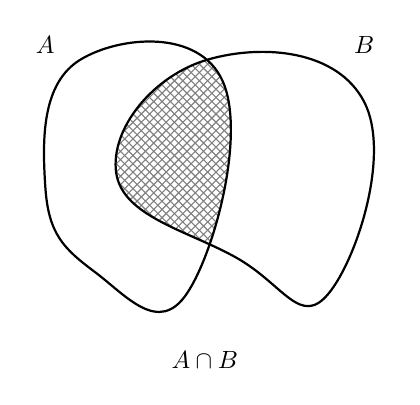
\begin{tikzpicture}[
        scale=0.9,
        transform shape,
        font=\sffamily,
        shaded/.style={
            pattern=crosshatch, 
            pattern color=gray
        }
    ]

    % Definição das formas
    \def\blobA{plot [smooth cycle, tension=0.8] coordinates {(-1.5,0) (-1,1.8) (1,1.5) (0.5,-1.5) (-0.8,-1.2)}}
    \def\blobB{plot [smooth cycle, tension=0.8] coordinates {(-0.5,0.2) (0.8,1.8) (3,1.2) (2.5,-1.5) (1.2,-1.0)}}

    % Interseção
    \begin{scope}[xshift=4cm]
        \begin{scope}
            \clip \blobA;
            \fill[shaded] \blobB;
        \end{scope}

        \draw[thick] \blobA;
        \draw[thick] \blobB;

        \node at (-1.5, 2) {\( A \)};
        \node at (3, 2) {\( B \)};

        \node[below, align=center] at (0.75, -2.2) {\( A \cap B \)};
    \end{scope}

    \end{tikzpicture}

    \fonte{Elaborado pelo autor (2025).}
\end{figure}

\begin{exemplo}[Existência da Interseção]
    Considere a fórmula \(\varphi\) dada por "\(x \in a\)". Aqui, \(a\) atua como um parâmetro (na notação do axioma, \(t_1 = a\)). O axioma correspondente a esta fórmula no Esquema de Separação é:
    \[
    \forall a \forall c \exists B \forall x (x \in B \iff x \in c \e x \in a)
    \]
    Este axioma garante que, dados dois conjuntos \(c\) e \(a\), existe um conjunto \(B\) contendo exatamente os elementos que pertencem a ambos. Esse conjunto \(B\) é a interseção \(c \cap a\).
\end{exemplo}

\begin{definicao}[Complemento Relativo; Diferença]
    Para quaisquer conjuntos \(A\) e \(B\), o complementar relativo de \(B\) em \(A\) (também chamado de diferença de conjuntos) é o conjunto \(A - B\) formado pelos elementos que pertencem a \(A\), mas não pertencem a \(B\).
    \[
    A - B = \{x \in A : x \notin B\}
    \]
    \label{def:complemento_relativo}
\end{definicao}

\begin{figure}[H]
    \centering
    \caption{Representação visual do Complemento Relativo}
    \label{fig:complemeto_relativo}
    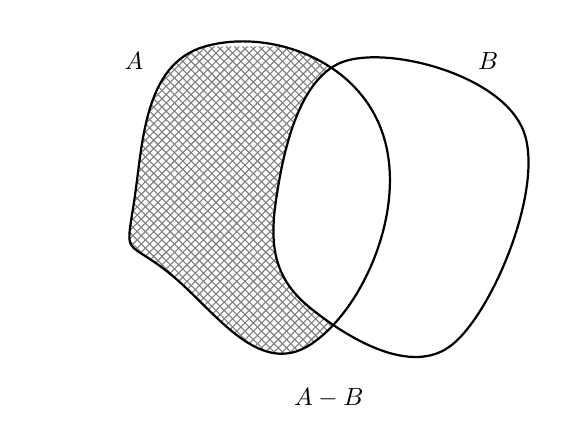
\begin{tikzpicture}[
        scale=0.9,
        transform shape,
        font=\sffamily,
        shaded/.style={
            pattern=crosshatch, 
            pattern color=gray
        }
    ]

    % Definição das formas
    \def\blobC{plot [smooth cycle, tension=0.9] coordinates {(-2,0) (-1, 2.2) (1.5, 1) (0.5, -2) (-1.5, -1)}}
    \def\blobD{plot [smooth cycle, tension=0.7] coordinates {(0,0) (1, 2) (3.5, 1) (2.5, -2) (0.5, -1.5)}}

    % Diferença (A - B)
    \begin{scope}[xshift=-8cm]
        
        \begin{scope}[even odd rule]
            \clip \blobD (-3.5,-2.2) rectangle (3.5,2.2);
            \clip \blobC;
            \fill[shaded] (-3.5,-2.2) rectangle (3.5,2.2);
        \end{scope}

        \draw[thick] \blobC;
        \draw[thick] \blobD;

        \node at (-2, 2) {\( A \)};
        \node at (3, 2) {\( B \)};
        \node[below, align=center] at (0.75, -2.5) {\( A - B \)};
    \end{scope}

    \end{tikzpicture}
    \fonte{Elaborado pelo autor (2025).}
\end{figure}

\begin{exemplo}[Existência do Complementar Relativo]
    Considere a fórmula \(\varphi\) dada por "\(x \notin a\)". Novamente, \(a\) é um parâmetro. O axioma gerado é:
    \[
    \forall a \forall c \exists B \forall x (x \in B \iff x \in c \e x \notin a)
    \]
    Este axioma assegura a existência do conjunto \(B\) formado pelos elementos que estão em \(c\) mas não estão em \(a\). Este conjunto é o complementar relativo de \(a\) em \(c\) (ou a diferença entre conjuntos), denotado por \(c - a\).
\end{exemplo}

\begin{exemplo}[O Conjunto de Russell Relativizado]
    Considere a fórmula \(\varphi\) dada por "\(x \notin x\)". Esta fórmula não possui parâmetros adicionais. O axioma resultante é:
    \[
    \forall c \exists B \forall x (x \in B \iff x \in c \e x \notin x)
    \]
    Este exemplo é historicamente crucial. Ele define o subconjunto \(B = \{x \in c : x \notin x\}\). Ao contrário da Teoria Ingênua, isso não gera uma contradição, mas sim prova que \(B \notin c\). Isso é usado para demonstrar que não existe um "conjunto de todos os conjuntos" \ (pois se \(c\) fosse tal conjunto, teríamos \(B \in c\) e chegaríamos ao Paradoxo de Russell).
\end{exemplo}

\begin{teorema}
    Não existe um conjunto ao qual todo conjunto pertença
    \[
    \nexists A \forall x (x \in A).
    \]
    \label{teo:conjunto_universo}
\end{teorema}

\begin{proof}
    Seja \(A\) um conjunto arbitrário, para mostrar que \(A\) não contém todos os conjuntos, basta construir um conjunto \(B\) não pertencente à \(A\). Seja
    \[
    B = \{x \in A: x \notin x\}.
    \]
    Nós temos por construção de \(B\) que 
    \[
    c \in B \iff c \in A \e c \notin c.
    \]
    Considere \(c = B\), então
    \[
    B \in B \iff B \in A \e B \notin B.
    \]
    Assuma que \(B \in A\), então a fórmula se reduz para
    \[
    B \in B \iff B \notin B.
    \]
    O que é uma contradição, pois para que um lado seja verdadeiro o outro precisa ser falso, logo o problema está em assumir que \(B \in A\), isso prova que \(B \notin A\).
\end{proof}

\begin{definicao}[União de Conjuntos]
    Suponha que temos uma coleção infinita de conjuntos \(A = \{b_0, b_1, b_2,\dots\}\) e queremos fazer a união de todos os \(b_i\). Precisamos de uma operação geral de união:
    \begin{align*}
        \bigcup A &= \bigcup_i b_i \\
        &= \{x: x \text{ é membro de algum elemento de } A\} \\
        &= \{x: (\exists b \in A)x \in b\}.
    \end{align*}
    \label{def:uniao}
\end{definicao}

\begin{exemplo}
    \begin{align*}
        \bigcup\{a,b\} &= \{x: x \text{ é elemento de algum membro de } \{a,b\}\} \\
        &= \{x: x \text{ é membro de } a \ou b\} \\
        &= a \cup b.
    \end{align*}
\end{exemplo}

\begin{exemplo}
    Em casos extremos nós temos
    \[\cup \{a\} = a \qquad \text{ e } \qquad \cup \varnothing = \varnothing.\]
\end{exemplo}

\begin{definicao}[Interseção de Conjuntos]
    Considere \(A\) como sendo o mesmo conjunto da \autoref{def:uniao}. Definimos a interseção \(\bigcap A\) de \(A\) como
    \[
    x \in \bigcap A \iff x \text{ é elemento de todo membro de } A.
    \]
    \label{def:intersecao}
\end{definicao}

\begin{figure}[H]
    \centering
    \caption{Representação visual da Interseção Infinita}
    \label{fig:intersecao_infinita}

    \begin{tikzpicture}[
        scale=0.9, 
        transform shape,
        font=\sffamily,
        shaded/.style={
            pattern=north west lines, 
            pattern color=gray!50
        }
    ]

    % Cores Condicionais
    \def\ColorSet{\ifbool{darkmode}{DarkModeLink}{LightModeLink}}
    \def\ColorInter{\ifbool{darkmode}{DarkModeViolet}{LightModeViolet}}

    % Definição das formas (Elipses rotacionadas representando b_i)
    \def\blobZero{(0,0) ellipse (3.5cm and 1.5cm)}
    \def\blobOne{plot [smooth cycle, tension=1] coordinates {(-2, -2) (2, -2) (2, 2) (-2, 2)}} % Círculo aproximado
    
    % Para simular a interseção de muitos, usamos rotações
    \newcommand{\drawSet}[2]{
        \draw[thick, \ColorSet, rotate=#1] (0,0) ellipse (3cm and 1.2cm);
        \node[\ColorSet, font=\footnotesize, rotate=#1] at (#1:3.2) {#2};
    }

    % Desenho dos conjuntos individuais (Coleção A)
    \drawSet{0}{\( b_0 \)}
    \drawSet{60}{\( b_1 \)}
    \drawSet{120}{\( b_2 \)}
    
    % Sugestão de mais conjuntos (Infinito)
    \draw[thin, \ColorSet!40, dashed, rotate=30] (0,0) ellipse (3cm and 1.2cm);
    \draw[thin, \ColorSet!40, dashed, rotate=90] (0,0) ellipse (3cm and 1.2cm);
    \draw[thin, \ColorSet!40, dashed, rotate=150] (0,0) ellipse (3cm and 1.2cm);

    % Área da Interseção (O "Miolo" comum a todos)
    % Recorte (Clip) sucessivo para isolar o centro
    \begin{scope}
        \clip (0,0) ellipse (3cm and 1.2cm); % Clip b0
        \clip [rotate=60] (0,0) ellipse (3cm and 1.2cm); % Clip b1
        \clip [rotate=120] (0,0) ellipse (3cm and 1.2cm); % Clip b2
        
        \fill[shaded] (-2,-2) rectangle (2,2);
        \draw[very thick, \ColorInter] (0,0) circle (0.6cm); % Aproximação visual da área resultante
    \end{scope}

    % Elemento x na Interseção
    \node[circle, fill=\ColorInter, inner sep=1.5pt] (x) at (0,0) {};
    \node[above right, text=\ColorInter, font=\bfseries] at (0,0) {\( x \)};

    % Elemento y fora (pertence a alguns, mas não a todos)
    \node[circle, inner sep=1.2pt] (y) at (2.65, 1) {};
    \node[right, font=\footnotesize] at (y) {\( y \notin \bigcap A \)};

    % Rótulo Explicativo
    \node[align=center, font=\small] at (0, -3.7) {
        \textbf{Interseção Total} \\
        \( \bigcap A = \{x: (\forall b \in A) x \in b\} \)
    };
    \draw[->, \ColorInter, dashed] (0, -3.2) -- (0, -0.7);

    \end{tikzpicture}

    \fonte{Elaborado pelo autor (2025).}
\end{figure}

\begin{teorema}
    Para qualquer conjunto não vazio \(A\), existe um único conjunto \(B\) t.q. para qualquer \(x\),
    \[
    x \in B \iff x \text{ é elemento de todos os membros de } A.
    \]
    \label{teo:intersecao_unica}
\end{teorema}

\begin{proof}
    Como \(A\) é não vazio, tome algum elemento \(c\) fixo de \(A\). Então por um \teref{ax:subconjunto}{Axioma de Subconjunto} existe um conjunto \(B\) t.q. para todo \(x\),
    \begin{align*}
        x \in B &\iff x \in c \e x \text{ é elemento de todo outro membro de } A \\
        &\iff x \text{ é elemento de todo membro de } A.  
    \end{align*}
    A unicidade segue do \autoref{ax:extensao}.
\end{proof}

O \autoref{teo:intersecao_unica} serve para definirmos \(\bigcap A\) como sendo esse conjunto \(B\). Temos também que 
\[
B = \{x: (\forall b \in A)x \in b\}.
\]

\begin{proposicao}
    Se \( b \in A \), então \( b \subseteq \bigcup A \).
    \label{prop:elemento_contido_uniao}
\end{proposicao}

\begin{proof}
    Seja \( x \) um elemento qualquer tal que \( x \in b \). Como \( b \in A \), pela definição de união de um conjunto de conjuntos, segue-se que \( x \in \bigcup A \). Portanto, todo elemento de \( b \) é um elemento de \( \bigcup A \), o que implica que \( b \subseteq \bigcup A \).
\end{proof}

\begin{proposicao}
    Se \( \{\{x\}, \{x, y\}\} \in A \), então \( \{x, y\} \in \bigcup A \), \( x \in \bigcup\bigcup A \) e \( y \in \bigcup\bigcup A \).
    \label{prop:ordenado_elemento_par_uniao}
\end{proposicao}

\begin{proof}
    Seja \( u = \{\{x\}, \{x, y\}\} \). Por hipótese, \( u \in A \). Visto que \( \{x, y\} \in u \), pela definição de união, temos que \( \{x, y\} \in \bigcup A \).
    
    Agora considere o conjunto \( \{x, y\} \). Como \( \{x, y\} \in \bigcup A \), qualquer elemento pertencente a \( \{x, y\} \) pertence a \( \bigcup(\bigcup A) \), denotado como \( \bigcup\bigcup A \).
    Como \( x \in \{x, y\} \), segue-se que \( x \in \bigcup\bigcup A \).
    De modo análogo, como \( y \in \{x, y\} \), segue-se que \( y \in \bigcup\bigcup A \).
\end{proof}

\begin{proposicao}
    Seja \( S = \{\{a\}, \{a, b\}\} \). Então \( \bigcup\bigcap S = a \) e \( \bigcap\bigcup S = a \cap b \).
    \label{prop:par_cupcap_capcup}
\end{proposicao}

\begin{proof}
    Primeiro, calculamos a interseção dos elementos de \( S \):
    \[
        \bigcap\{\{a\}, \{a, b\}\} = \{a\} \cap \{a, b\} = \{a\}
    \]
    Logo, aplicando a operação de união ao resultado:
    \[
        \bigcup\bigcap\{\{a\}, \{a, b\}\} = \bigcup\{a\} = a
    \]
    Por outro lado, calculamos primeiro a união dos elementos de \( S \):
    \[
        \bigcup\{\{a\}, \{a, b\}\} = \{a\} \cup \{a, b\} = \{a, b\}
    \]
    Portanto, aplicando a operação de interseção ao resultado (assumindo que \( a \) e \( b \) são conjuntos):
    \[
        \bigcap\bigcup\{\{a\}, \{a, b\}\} = \bigcap\{a, b\} = a \cap b
    \]
\end{proof}

\begin{proposicao}
    Se todo membro de \(\mathcal{A}\) é um subconjunto de \(B\), então \(\bigcup \mathcal{A} \subseteq B\)
    \[
    (a \in \AA \implies a \sub B) \implies \bigcup \AA \sub B.
    \]
    \label{prop:uniao_familia_subconjunto}
\end{proposicao}

\begin{proof}
    Para provar que \(\bigcup \AA \sub B\) precisamos mostrar que para qualquer \(x \in \bigcup \AA\) necessariamente \(x \in B\). Pela \autoref{def:uniao}, \(x \in \bigcup \AA \iff \exists a \in \AA \tq x \in a\).
    \begin{align*}
        x \in \bigcup \AA &\implies \exists a \in \AA \tq x \in a, \\
        a \in \AA &\implies a \sub B, \\
        x \in a \sub B &\implies x \in B.
    \end{align*}
\end{proof}

\begin{proposicao}
    Para todo conjunto \(A\), tem-se que \(\bigcup \PP(A) = A\).
    \label{prop:uniao_partes_identidade}
\end{proposicao}

\begin{proof}
    Devemos demonstrar a dupla inclusão entre os conjuntos.
    
    (\(\subseteq\)) Seja \(x \in \bigcup \PP(A)\). Pela definição de união, existe algum \(S \in \PP(A)\) tal que \(x \in S\). Pela definição de conjunto das partes, \(S \in \PP(A) \implies S \sub A\). Logo, se \(x \in S\) e \(S \sub A\), então necessariamente \(x \in A\).
    
    (\(\supseteq\)) Seja \(x \in A\). Sabemos que \(A \sub A\), logo \(A \in \PP(A)\). Como existe um conjunto em \(\PP(A)\) (o próprio \(A\)) que contém \(x\), concluímos por definição que \(x \in \bigcup \PP(A)\).
    
    Portanto, vale a igualdade \(\bigcup \PP(A) = A\).
\end{proof}

\begin{proposicao}
    Para todo conjunto \(A\), vale a inclusão \(A \subseteq \PP(\bigcup A)\). A igualdade \(A = \PP(\bigcup A)\) ocorre se, e somente se, existe um conjunto \(B\) tal que \(A = \PP(B)\) (ou seja, se \(A\) é um conjunto das partes).
    \label{prop:inclusao_A_partes_uniao}
\end{proposicao}

\begin{proof}
    Seja \(x \in A\). Para demonstrar que \(x \in \PP(\bigcup A)\), devemos mostrar que \(x \sub \bigcup A\).
    
    Tome um elemento arbitrário \(y \in x\). Visto que \(y \in x\) e \(x \in A\), pela definição de união, temos que \(y \in \bigcup A\).
    
    Como a escolha de \(y\) foi arbitrária, concluímos que todo elemento de \(x\) pertence a \(\bigcup A\), ou seja, \(x \sub \bigcup A\).
    
    Finalmente, pela definição de conjunto das partes, \(x \sub \bigcup A \implies x \in \PP(\bigcup A)\). Portanto, \(A \sub \PP(\bigcup A)\).

    A demonstração da igualdade fica a cargo do leitor.
\end{proof}

\begin{proposicao}
    Para quaisquer conjuntos \(A\) e \(B\), \(\PP(A) \cap \PP(B) = \PP(A \cap B)\).
    \label{prop:intersecao_partes}
\end{proposicao}

\begin{proof}
    Para demonstrar a igualdade, mostraremos que um conjunto qualquer pertence ao lado esquerdo se, e somente se, pertence ao lado direito.

    Seja \(S\) um conjunto qualquer. Temos que:
    \begin{align*}
        S \in \PP(A) \cap \PP(B) &\iff S \in \PP(A) \text{ e } S \in \PP(B) \\
        &\iff S \sub A \text{ e } S \sub B \\
        &\iff S \sub (A \cap B) \\
        &\iff S \in \PP(A \cap B).
    \end{align*}
    
    Portanto, \(\PP(A) \cap \PP(B) = \PP(A \cap B)\).
\end{proof}

\begin{proposicao}
    Para quaisquer conjuntos \(A\) e \(B\), vale a inclusão \(\PP(A) \cup \PP(B) \subseteq \PP(A \cup B)\). A igualdade ocorre se, e somente se, \(A \subseteq B\) ou \(B \subseteq A\).
    \label{prop:uniao_partes_inclusao}
\end{proposicao}

\begin{proof}
    Seja \(S \in \PP(A) \cup \PP(B)\). Pela definição de união, temos que \(S \in \PP(A)\) ou \(S \in \PP(B)\). Analisaremos os dois casos:
    \begin{itemize}
        \item Se \(S \in \PP(A)\), então \(S \sub A\). Como sabemos que \(A \sub A \cup B\), pela transitividade da inclusão temos \(S \sub A \cup B\). Logo, \(S \in \PP(A \cup B)\).
        \item Analogamente, se \(S \in \PP(B)\), então \(S \sub B\). Como \(B \sub A \cup B\), segue que \(S \sub A \cup B\). Logo, \(S \in \PP(A \cup B)\).
    \end{itemize}
    Em qualquer caso, concluímos que \(S \in \PP(A \cup B)\). Portanto, a inclusão \(\PP(A) \cup \PP(B) \sub \PP(A \cup B)\) é válida.
    
    A demonstração da igualdade é deixada a cargo do leitor.
\end{proof}

\begin{proposicao}
    Não existe um conjunto ao qual pertença todo \textit{singleton} (ou seja, todo conjunto da forma \(\{x\}\)).
    \label{prop:inexistencia_conjunto_unitarios}
\end{proposicao}

\begin{proof}
    Suponha, por absurdo, que exista um conjunto \(\AAA\) que contenha todos os \textit{singletons}. Ou seja, para qualquer conjunto \(x\), temos que \(\{x\} \in \AAA\).
    
    Considere agora o conjunto \(\bigcup \AAA\). Dado um conjunto qualquer \(y\), podemos formar o conjunto unitário \(\{y\}\). Pela nossa hipótese, \(\{y\} \in \AAA\).
    
    Pela definição de união, \(z \in \bigcup \AAA \iff \exists S \in \AAA \tq z \in S\). Como \(\{y\} \in \AAA\) e \(y \in \{y\}\), conclui-se que \(y \in \bigcup \AAA\).
    
    Visto que \(y\) é um conjunto arbitrário, isso implica que \(\bigcup \AAA\) contém todos os conjuntos existentes. Portanto, \(\bigcup \AAA\) seria o conjunto de todos os conjuntos, cuja existência entra em contradição com o \autoref{teo:conjunto_universo}.
    
    Essa contradição mostra que tal conjunto \(\AAA\) não pode existir.
\end{proof}

\begin{proposicao}
    Se \(a \in B\), então \(\PP(a) \in \PP(\PP(\bigcup B))\).
    \label{prop:inclusao_partes_duplo}
\end{proposicao}

\begin{proof}
    A demonstração segue da aplicação sucessiva das definições de união e conjunto das partes.
    
    Primeiro, observe que \(a \sub \bigcup B\). De fato, se \(x \in a\), como \(a \in B\), então \(x\) pertence a um conjunto que está em \(B\), o que implica \(x \in \bigcup B\).
    
    Agora, mostraremos que \(\PP(a) \sub \PP(\bigcup B)\). Seja \(S \in \PP(a)\). Então \(S \sub a\). Como \(a \sub \bigcup B\), pela transitividade da inclusão, temos \(S \sub \bigcup B\). Logo, \(S \in \PP(\bigcup B)\).
    
    Visto que todo elemento de \(\PP(a)\) é também elemento de \(\PP(\bigcup B)\), concluímos que \(\PP(a) \sub \PP(\bigcup B)\).
    
    Finalmente, pela definição de conjunto das partes, se \(\PP(a) \sub \PP(\bigcup B)\), então \(\PP(a) \in \PP(\PP(\bigcup B))\).
\end{proof}

\begin{proposicao}
    A diferença de conjuntos não é associativa. Isto é, existem conjuntos \(A\), \(B\) e \(C\) tais que \(A - (B - C) \neq (A - B) - C\).
    \label{prop:diferenca_nao_associativa}
\end{proposicao}

\begin{definicao}[Diferença Simétrica]
    A diferença simétrica \(A + B\) dos conjuntos \(A\) e \(B\) é o conjunto definido por \((A - B) \cup (B - A)\).
    \label{def:diferenca_simetrica}
\end{definicao}

\begin{figure}[H]
    \centering
    \caption{Representação visual da Diferença Simétrica}
    \label{fig:diferenca_simetrica}
    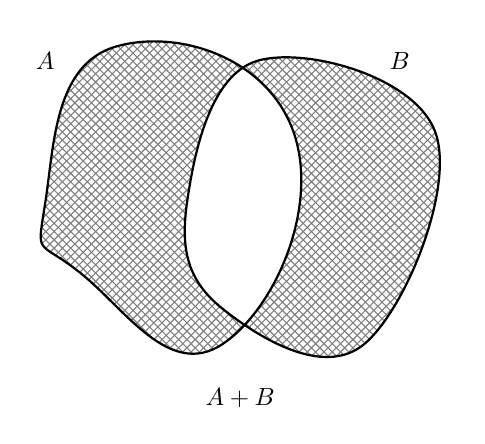
\begin{tikzpicture}[
        scale=0.9,
        transform shape,
        font=\sffamily,
        shaded/.style={
            pattern=crosshatch, 
            pattern color=gray
        }
    ]

    \usetikzlibrary{patterns}

    % Definição das formas
    \def\blobC{plot [smooth cycle, tension=0.9] coordinates {(-2,0) (-1, 2.2) (1.5, 1) (0.5, -2) (-1.5, -1)}}
    \def\blobD{plot [smooth cycle, tension=0.7] coordinates {(0,0) (1, 2) (3.5, 1) (2.5, -2) (0.5, -1.5)}}

    % Diferença Simétrica (A + B)
    \begin{scope}

        \fill[shaded, even odd rule] \blobC \blobD;

        \draw[thick] \blobC;
        \draw[thick] \blobD;

        \node at (-2, 2) {\( A \)};
        \node at (3, 2) {\( B \)};
        \node[below, align=center] at (0.75, -2.5) {\( A + B \)};
    \end{scope}

    \end{tikzpicture}
    \fonte{Elaborado pelo autor (2025).}
\end{figure}

\begin{proposicao}
    Para quaisquer conjuntos \(A\), \(B\) e \(C\), a interseção é distributiva em relação à diferença simétrica:
    \[ A \cap (B + C) = (A \cap B) + (A \cap C) \]
    \label{prop:distributividade_simetrica}
\end{proposicao}

\begin{proposicao}
    Para quaisquer conjuntos \(A\), \(B\) e \(C\), a diferença simétrica é associativa:
    \[ A + (B + C) = (A + B) + C \]
    \label{prop:associatividade_simetrica}
\end{proposicao}

\begin{proposicao}
    Para quaisquer conjuntos \(A\) e \(B\), as seguintes quatro condições são equivalentes:
    \begin{enumerate}
        \item[(a)] \(A \subseteq B\);
        \item[(b)] \(A - B = \varnothing\);
        \item[(c)] \(A \cup B = B\);
        \item[(d)] \(A \cap B = A\).
    \end{enumerate}
    \label{prop:condicoes_equivalentes_inclusao}
\end{proposicao}

\begin{proposicao}
    Sejam \(A\), \(B\) e \(C\) conjuntos tais que \(A \cup B = A \cup C\) e \(A \cap B = A \cap C\). Então, \(B = C\).
    \label{prop:unicidade_por_uniao_e_intersecao}
\end{proposicao}

\begin{proposicao}
    Para quaisquer famílias de conjuntos \(A\) e \(B\), tem-se que:
    \[ \bigcup(A \cup B) = \bigcup A \cup \bigcup B \]
    \label{prop:uniao_da_uniao_de_familias}
\end{proposicao}

\begin{proposicao}
    Se \(A\) e \(B\) são famílias não vazias de conjuntos, então:
    \[ \bigcap(A \cup B) = \bigcap A \cap \bigcap B \]
    \label{prop:intersecao_da_uniao_de_familias}
\end{proposicao}

\begin{proposicao}
    Se \(\mathscr{B}\) é uma família não vazia de conjuntos, então a união distribui sobre a interseção da seguinte forma:
    \[ A \cup \bigcap \mathscr{B} = \bigcap \{ A \cup X: X \in \mathscr{B} \} \]
    \label{prop:distributiva_uniao_intersecao_familia}
\end{proposicao}

\begin{proposicao}
    Se \(\mathscr{A}\) é uma família não vazia de conjuntos, então o conjunto das partes da interseção é igual à interseção dos conjuntos das partes:
    \[ \PP(\bigcap \mathscr{A}) = \bigcap \{ \PP(X): X \in \mathscr{A} \} \]
    \label{prop:partes_intersecao_familia}
\end{proposicao}

\begin{proposicao}
    Para qualquer família de conjuntos \(\mathscr{A}\), a união dos conjuntos das partes está contida no conjunto das partes da união:
    \[ \bigcup \{ \PP(X): X \in \mathscr{A} \} \subseteq \PP(\bigcup \mathscr{A}) \]
    A igualdade ocorre se, e somente se, \(\bigcup \mathscr{A} \in \mathscr{A}\) (ou seja, existe um conjunto \(M \in \mathscr{A}\) tal que todos os outros membros de \(\mathscr{A}\) são subconjuntos de \(M\)).
    \label{prop:uniao_partes_inclusao_familia}
\end{proposicao}

\begin{proposicao}
    A igualdade
    \[ A \cup \bigcup \mathscr{B} = \bigcup \{ A \cup X: X \in \mathscr{B} \} \]
    é válida se, e somente se, a família \(\mathscr{B}\) não for vazia (ou se \(A\) for vazio). Caso \(\mathscr{B} = \varnothing\) e \(A \neq \varnothing\), a igualdade não se verifica.
    \label{prop:distributiva_uniao_familia_condicao}
\end{proposicao}

\hrule

\begin{axioma}[Esquema de Axiomas de Substituição]
    Para cada fórmula \(\varphi(x,y)\) que não contenha o símbolo \(B\), a seguinte sentença é um axioma:
    \begin{align*}
        \forall A [(\forall x \in A) \forall y_1 \forall y_2 (\varphi(x, y_1) \e \varphi(x, y_2) \implies y_1 = y_2) \\
    \implies \exists B \forall y (\exists y \in B \iff (\exists x \in A)\varphi(x, y))].
    \end{align*}
    \label{ax:substituicao}
\end{axioma}

\begin{axioma}[Axioma do Infinito]
    Existe um conjunto indutivo:
    \[ (\exists A)[\varnothing \in A \e (\forall a \in A) a^{+} \in A]. \]
    \label{ax:infinito}
\end{axioma}

\begin{axioma}[Axioma da Regularidade]
    Todo conjunto não vazio $A$ possui um membro $m$ tal que $m \cap A =\varnothing$:
    \[ 
    (\forall A \neq \varnothing)(\exists m \in A)m \cap A = \varnothing.
    \]
    \label{ax:regularidade}
\end{axioma}

\section{Álgebra de Conjuntos}
\label{sec:algebra_conjuntos}

Para iniciar essa seção, relembramos as operações básicas de conjuntos já definidas:

\begin{align*}
    &\text{União} &A \cup B = \{x: x \in A \ou x \in B\}, \\
    &\text{Interseção} &A \cap B = \{x: x \in A \e x \in B\}, \\
    &\text{Complemento Relativo} &A - B = \{x \in A: x \notin B\}, \\
    &\text{Diferença Simétrica} &A + B = \{x \in A \cup B: x \notin A \cap B\}.
\end{align*}

As seguintes propriedades são fundamentais para a álgebra de conjuntos, as demonstrações ficam a cargo do leitor:

Comutatividade:

\begin{align*}
    A \cup B = B \cup A, \\
    A \cap B = B \cap A.
\end{align*}

Associatividade:

\begin{align*}
    A \cup (B \cup C) = (A \cup B) \cup C, \\
    A \cap (B \cap C) = (A \cap B) \cap C. \\
\end{align*}

Distributiva:

\begin{align*}
    A \cup \bigcap B = \bigcap \{A \cup x: x \in B\}, \\
    A \cap \bigcup B = \bigcup \{A \cap x: x \in B\}.
\end{align*}

Leis de De Morgan:

\begin{align*}
    C - (A \cup B) = (C - A) \cap (C - B), \\
    C - (A \cap B) = (C - A) \cup (C - B).
\end{align*}

Identidades Com \(\varnothing\):

\begin{align*}
    A \cup \varnothing = A, \\
    A \cap \varnothing = \varnothing, \\
    A \cap (C - A) = \varnothing.
\end{align*}

\begin{remark}
    Muitas vezes quando trabalhando Com Conjuntos, estaremos Apenas trabalhando Com subconjuntos de um "espaço" \ maior \(E\), nesses Casos, podemos Abreviar \(E - A\) Apenas Como \(-A\).
\end{remark}

Considerando um espaço \(E\) nós temos As seguintes identidades:

\begin{align*}
    A \cup E = E \qquad \text{ e } \qquad A \cap E = A, \\
    A \cup -A = E \qquad \text{ e } \qquad A \cap -A = \varnothing. 
\end{align*}

Para a relação de inclusão, temos as seguintes propriedades monótonas\footnote{Refere-se a operações que preservam a ordem.}:

\begin{align*}
    A \subseteq B \implies A \cup C \subseteq B \cup C, \\
    A \subseteq B \implies A \cap C \subseteq B \cap C, \\
    A \subseteq B \implies \bigcup A \subseteq \bigcup B,
\end{align*}
e as propriedades antimonótonas\footnote{Refere-se a operações que não preservam a ordem.}: 

\begin{align*}
    A \subseteq B \implies C - B \subseteq C - A, \\
    \varnothing \neq A \subseteq B \implies \bigcap B \subseteq \bigcap A.
\end{align*}

\section{Relações e Funções}
\label{sec:relacoes_funcoes}

\begin{definicao}[Par Ordenado]
    Definimos o par ordenado \((a,b)\) onde a primeira coordenada de \((a,b)\) é \(a\) e a segunda coordenada de \((a,b)\) é \(b\) como
    \[
    (a,b) = \{\{a\}, \{a,b\}\}.
    \] 
    \label{def:par_ordenado}
\end{definicao}

\begin{teorema}
    Os pares ordenados \((u,v)\) e \((x,y)\) são iguais se, e somente se, \(u=x\) e \(v=y\)
    \[
    (u,v) = (x,y) \iff u = x \text{ e } v = y.
    \]
    \label{teo:par_ordenado}
\end{teorema}

\begin{proof} 
    \begin{adjustwidth}{1cm}{0cm}
        \begin{enumerate}
        \item[\((\impliedby)\)] Trivial.
        \item[\((\implies)\)] Assuma que \((u,v) = (x,y)\), então 
        \[
        \{\{u\}, \{u,v\}\} = \{\{x\}, \{x,y\}\}.
        \]
        Disso temos 
        \[
        (1) \ \{u\} \in \{\{x\}, \{x,y\}\} \qquad \text{ e } \qquad (2) \ \{u,v\} \in \{\{x\}, \{x,y\}\}.
        \]
        De \((1)\) temos que 
        \[
        (a) \ \{u\} = \{x\} \qquad \ou \qquad (b) \ \{u\} = \{x,y\},
        \]
        de \((2)\) temos que
        \[
        (c) \ \{u,v\} = \{x\} \qquad \ou \qquad (d) \ \{u,v\} = \{x,y\}.
        \] 
        Precisamos analisar caso a caso, assumindo cada um como verdadeiro:
        \begin{enumerate}
            \item[(b)] Suponha  (b) verdadeiro. Então $u = x = y$. Logo (c) e (d) são equivalentes e nos dizem que $u = v = x = y$. Neste caso, a conclusão do teorema é válida.
            \item[(c)] Análogo a (b).
            \item[(a)] Suponha (a) verdadeiro. Temos $u = x$. De (d), obtemos que $u = y$ ou $v = y$. No primeiro caso, (b) é válida, esse caso já foi considerado. No segundo caso, temos $v = y$, como desejado.
            \item[(d)] Análogo a (a).   
        \end{enumerate}
    \end{enumerate}
    \end{adjustwidth}
\end{proof}

\begin{definicao}[Produto Cartesiano]
    Sejam \(A\) e \(B\) conjuntos, podemos fazer pares ordenados \((x,y)\) com \(x \in A\) e \(y \in B\). A coleção de todos esses pares é o Produto Cartesiano \(A \times B\) de \(A\) e \(B\):
    \[
    A \times B = \{(x,y): x \in A \e y \in B\}.
    \]
    \label{def:produto_cartesiano}
\end{definicao}

\begin{figure}[H]
    \centering
    \caption{Representação visual do Produto Cartesiano \( A \times B \)}
    \label{fig:produto_cartesiano}

    \begin{tikzpicture}[
        scale=0.9,
        transform shape,
        font=\sffamily,
        shaded/.style={
            pattern=north west lines, 
            pattern color=gray!50
        }
    ]

    \usetikzlibrary{patterns, positioning}

    % Definição das Formas
    
    % Conjunto A (Horizontal)
    \def\blobA{plot [smooth cycle, tension=0.7] coordinates {(0,-0.5) (4,-0.5) (4.2,-1.5) (2,-1.8) (-0.2,-1.5)}}
    
    % Conjunto B (Vertical)
    \def\blobB{plot [smooth cycle, tension=0.7] coordinates {(-0.5,0) (-1.5,0) (-1.8,2) (-1.5,3.5) (-0.5,3.5)}}

    % Área do Produto (AxB)    
    \def\blobProduct{plot [smooth cycle, tension=0.8] coordinates {(0.2, 0.2) (3.8, 0.5) (3.5, 3.2) (0.5, 3.5) (-0.2, 1.8)}}

    % Desenho da Área do Produto
    \begin{scope}[xshift=0.5cm]
    \fill[shaded] \blobProduct;    
    \draw[gray, dashed, thick] \blobProduct;   
    \node[] at (4.8, 3) {\( A \times B \)};      
    \end{scope}

    % Desenho dos Conjuntos Origem
    
    % Conjunto A (Embaixo)
    \draw[thick] \blobA;
    \node at (2, -1.2) {\Large \( A \)};
    
    % Conjunto B (Na esquerda)
    \draw[thick] \blobB;
    \node at (-1, 1.75) {\Large \( B \)};

    % Elementos e Projeções
    
    % Elemento x em A
    \node[circle, fill=\ifbool{darkmode}{DarkModeLink}{LightModeLink}, inner sep=1.5pt, label={below:\textcolor{\ifbool{darkmode}{DarkModeLink}{LightModeLink}}{\( x \)}}] (x) at (1.5, -0.9) {};
    
    % Elemento y em B
    \node[circle, fill=\ifbool{darkmode}{DarkModeRed}{LightModeRed}, inner sep=1.5pt, label={left:\textcolor{\ifbool{darkmode}{DarkModeRed}{LightModeRed}}{\( y \)}}] (y) at (-1, 3) {};

    % O Par Ordenado (x,y) dentro da área do produto
    \node[circle, fill=black, inner sep=1.5pt, label={right:\( (x,y) \)}] (pair) at (1.8, 2.2) {};

    % Linhas de projeção curvas
    \draw[dashed, thin, \ifbool{darkmode}{DarkModeLink}{LightModeLink}, ->, >=latex] (x) to[out=90, in=-90] (pair);
    \draw[dashed, thin, \ifbool{darkmode}{DarkModeRed}{LightModeRed}, ->, >=latex] (y) to[out=0, in=180] (pair);

    \end{tikzpicture}

    \fonte{Elaborado pelo autor (2025).}
\end{figure}

\begin{lema}
    Se \(x \in C\) e \(y \in C\), então \((x,y) \in \PP(\PP(C))\)
    \[
    (x \in C \e y \in C) \implies (x,y) \in \PP(\PP(C)).
    \]
    \label{lema:power_power}
\end{lema}

\begin{proof}
    Suponha que $x \in C$ e $y \in C$. Pela \autoref{def:par_ordenado}, o par ordenado $(x,y)$ é o conjunto $\{\{x\}, \{x,y\}\}$.
    
    Para mostrar que $\{\{x\}, \{x,y\}\} \in \PP(\PP(C))$, devemos mostrar que $\{\{x\}, \{x,y\}\} \subseteq \PP(C)$, o que exige que $\{x\} \in \PP(C)$ e $\{x,y\} \in \PP(C)$. Analisamos os dois elementos:
    
    \begin{enumerate}
        \item Como $x \in C$, o \textit{singleton} $\{x\}$ é um subconjunto de $C$ ($\{x\} \subseteq C$). Pela definição de conjunto das partes, isso implica que $\{x\} \in \PP(C)$.
        \item Como $x \in C$ e $y \in C$, o conjunto par $\{x,y\}$ é um subconjunto de $C$ ($\{x,y\} \subseteq C$). Logo, $\{x,y\} \in \PP(C)$.
    \end{enumerate}
    
    Visto que ambos os elementos de $(x,y)$ pertencem a $\PP(C)$, concluímos que $(x,y) \subseteq \PP(C)$. Portanto, pela definição de conjunto das partes aplicada novamente, $(x,y) \in \PP(\PP(C))$.
\end{proof}

\begin{corolario}
    Para quaisquer conjuntos \(A\) e \(B\), existe um conjunto no qual seus elementos são exatamente os pares ordenados \((x,y)\) com \(x \in A\) e \(y \in B\)
    \[
    \forall A \forall B \exists C \forall z (z \in C \iff \exists x \exists y (x \in A \e y \in B \e z = (x,y))).
    \]
    \label{cor:existencia_par_odernado}
\end{corolario}

\begin{proof}
    De um Axioma de \autoref{ax:subconjunto} nós podemos construir o conjunto
    \[
    \AAA = \{w \in \PP(\PP(A \cup B)): \exists x \in A \e \exists y \in B \tq w = (x,y) \}.
    \]
    Como \(x \in A \cup B\) e \(y \in A \cup B\), temos pelo \autoref{lema:power_power} que \(\{\{x\}, \{x,y\}\} \in \PP(\PP(A \cup B))\), ou seja, \((x,y) \in \PP(\PP(A \cup B))\), assim sabemos que todos os pares ordenados \((x,y)\) com \(x \in A\) e \(y \in B\) estão em \(\PP(\PP(A \cup B))\), precisamos agora garantir que apenas pares ordenados fazem parte de \(\AAA\). Pela construção de \(\AAA\) temos que 
    \[
    w \in \AAA \iff w = (x,y) \text{ para algum } x \in A \text{ e algum } y \in B,
    \]
    ou seja, \(w\) está em \(\AAA\) se, e somente se é um par ordenado com \(x \in A\) e \(y \in B\).
\end{proof}



\section{Conjunto dos Números Naturais}
\label{sec:numeros_naturais}

O ponto de partida para a construção dos números é o conjunto dos números naturais, \(\mathbb{N} = \{0, 1, 2, 3, ...\}\), caracterizado pelos axiomas de Peano:

\begin{axioma}[Primeiro Axioma de Peano]
    Existe uma função injetiva \(s: \ \mathbb{N} \to \mathbb{N}.\) Chamamos a imagem de \(s(n)\) de sucessor de \(n\).
    \label{ax:peano1}    
\end{axioma}

\begin{axioma}[Segundo Axioma de Peano]
    Existe um único número natural \(0 \in \mathbb{N}\) tal que \(0 \neq s(n)\) para qualquer \(n \in \mathbb{N}\).
    \label{ax:peano2}
\end{axioma}

\begin{axioma}[Terceiro Axioma de Peano]
    Se em um conjunto \(X \subseteq \mathbb{N}\), \(0 \in X\) e \(s(X) \subseteq X\)\footnote{\(n \in X \implies s(n) \in X.\)}, então \(X = \mathbb{N}\).  
    \label{ax:peano3}
\end{axioma}
Esses axiomas estabelecem a existência de um \textbf{primeiro elemento} (que chamamos de \(1\)), uma função "\textbf{sucessor}" \ injetiva, e o \textbf{princípio da indução}, que garante que qualquer número natural pode ser alcançado a partir do \(1\) por sucessivas aplicações da função sucessor.

\begin{definicao}[Sucessor]
    Definimos o sucessor de um número \(x\) como 
    \[
    x^+ = x \cup \{x\}
    \]
    \label{def:funcao-sucessor}
\end{definicao}

